\documentclass[10pt]{beamer}

\usetheme[progressbar=frametitle]{metropolis}
\usepackage{appendixnumberbeamer}

\usepackage{booktabs}
\usepackage[scale=2]{ccicons}

\usepackage{pgfplots}
\usepgfplotslibrary{dateplot}

\usepackage{xspace}
\newcommand{\themename}{\textbf{\textsc{metropolis}}\xspace}

\usepackage{blindtext}
\usepackage{multirow}
\usepackage{amsmath}
\usepackage{threeparttable}
\usepackage{booktabs}
\usepackage{tabularx}
\usepackage{graphicx}
\usepackage{subfig}

\newcolumntype{L}[1]{>{\raggedright\arraybackslash}p{#1}} % linksbündig mit Breitenangabe
\newcolumntype{C}[1]{>{\centering\arraybackslash}p{#1}} % zentriert mit Breitenangabe
\newcolumntype{R}[1]{>{\raggedleft\arraybackslash}p{#1}} % rechtsbündig mit Breitenangabe

\usepackage[
    backend=biber,
    style=bwl-FU,
    url=false,
    doi=false,
    eprint=false
]{biblatex}
\addbibresource{Biblio.bib}

\title{Beamer Test}
\subtitle{A Discussion on important Topics}
\date{\today}
\author{Tobias Klöpper, Michele M. Senkal, Marco Barcellos and David Annoni}
\institute{Institute for Brewing and Degustation}
% \titlegraphic{\hfill\includegraphics[height=1.5cm]{logo.pdf}}

\begin{document}

\maketitle

\begin{frame}{Table of contents}
  \setbeamertemplate{section in toc}[sections numbered]
  \tableofcontents%[hideallsubsections]
\end{frame}

\section{Lorem ipsum}
\begin{frame}{Lorem ipsum}
\blindtext
\end{frame}

\section{Figures and Tables}
\begin{frame}{Tables}
The following Table \ref{table:1} shows a list of beers and my assessment of them.
\begin{table}[h!]
\begin{tabular}{ |p{3cm}||p{3cm}|p{2cm}|p{1cm}|  }
 \hline
 \multicolumn{4}{|c|}{Beer Ratings} \\
 \hline
 Beer Name & Country of Origin &Type of beer&Rating\\
 \hline
 Krombacher   & Germany    & Pils &   6/10\\
 Oettinger&   Germany  & Export   &10/10\\
 Feldschlösschen &Switzerland & Lager &  5/10\\
 Heineken    &Netherlands & Lager &  5/10\\
 Pilsner Urquell&   Czech Republic  & Pils & 7/10\\
 Arany Àszok& Hungary  & Lager   & 2/10\\
 Dreher& Hungary  & Pils & 5/10\\
 \hline
 \end{tabular}
 \caption{Own assessment of beers}
 \label{table:1}
\end{table}
\end{frame}



\begin{frame}{Table 2}
\begin{table}[h]
\begin{center}
\begin{threeparttable}
\begin{tabular}{c c c c}
    \toprule
    \textbf{Beer Name} & \textbf{Country of Origin} & \textbf{Type of Beer} & \textbf{Rating} \\ 
    \midrule
      Oettinger Export\tnote{1}   & Germany & Pils & 10/10 \\
      Oettinger Pils\tnote{2}   & Germany & Export & 2/10 \\ 
      \bottomrule
\end{tabular}
\begin{tablenotes}
\item[1] \footnotesize actually quite pleasant, even cheaply attainable in Kiosks for about 1€; \item[2] \footnotesize only consume ice cold, tastes way better after you already had a couple of beers
\end{tablenotes}
\end{threeparttable}
\end{center}
\caption{Beer Ratings with new packages}{}
\label{table:2}
\end{table}
\end{frame}

\begin{frame}{Table 3}
\begin{table}[h]
\centering
\begin{tabular}{llr}
\hline
\multicolumn{2}{c}{Item} \\
\cline{1-2}
Types    & Origin & Price (\$) \\
\hline
Red wine      & Tuscany     & 99.99      \\
White wine       & Bordeaux     & 20.50      \\
Rosé       & Valais     & 5.95      \\
Pinot Noir & Ticino      & 25.00       \\
\hline
\end{tabular}
\caption{EU origin protected wine list}
 \label{table:3}
\end{table}
\end{frame}

\begin{frame}{Important Equations}
\framesubtitle{Using package amsmath}
	\begin{gather}
	  	e^{\pi i}  - 1 = 0 \\
	 	 g = 10 m/s^2
	\end{gather}
\end{frame}

\begin{frame}{Slide with Proof}
\framesubtitle{Using the Theorem Environment}

	\begin{theorem}
	Let \(f\) be a function whose derivative exists in every point, then \(f\) 
	is a continuous function.
	\end{theorem}
	See figure \ref{figure1}:

	\begin{figure}
		\centering 
		\subfloat[\centering Bad Function]{{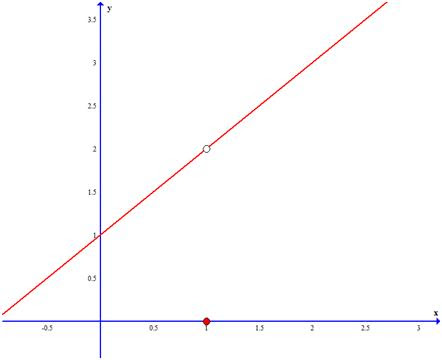
\includegraphics[width = 3cm]{figure.jpg} }}
		\qquad
		\subfloat[\centering Good Function]{{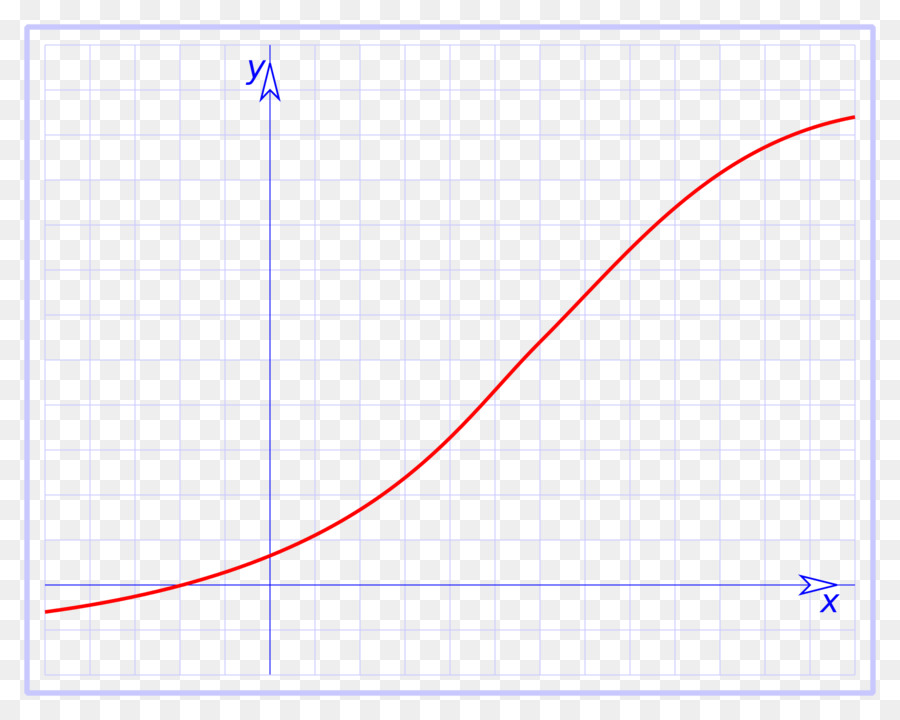
\includegraphics[width = 3cm]{figure2.jpg} }}
		\caption{Good and Bad functions}
		\label{figure1}
	\end{figure}

\end{frame}


\section{Discussion}
\setbeamertemplate{frame footer}{This is a custom footer test} %applies to a section so References are also including footer
\begin{frame}{Discussion}
Even though \cite{Zhao2015} suggest that "chitooligosaccharide should be an excellent preservative to inhibit beer-spoilage bacteria in the brewing process and in the end product" , we are not quite convinced that it will not interfere with the Reinheitsgebot. On the other hand we discovered that Charles \cite{Beer2003} does not seem to have any connection to this subject even though his name suggests so.
\end{frame} 


\begin{frame}[allowframebreaks]{References}

\printbibliography

\end{frame}

\end{document}